\newpage
\section*{Zielsetzung}
Aufnehmen und analysieren von dem Emissionsspektrum einer CU-
Röntgenröhre und verschiedener Absorbtionsspektren.
\section{Theorie}
\subsection{Erzeugung Röntgenstrahlung}
Innerhalb einer evakuierten Röhre werden Elektronen aus einer Glühkathode
auf eine Anode hin beschleunigt.\\ 
Die Energie der Strahlung kann mithilfe der Bragg-Reflexion ermittelt werden.
Durch Beugung an einem dreidimsensionalen Gitter (LiF-Kristall) mit der Gitterkonstante $d$ 
entsteht eine konstruktive Interferenz bei einem Braggwinkel $\Theta$. Durch die Bragg-Bedingung
\begin{equation}
    2 d sin(\Theta)=n\lambda,
    \label{eqn:bragg}
\end{equation}
ergibt sich die Wellenlänge. n ist dabei die Beugungsordunung.
\begin{figure}
    \centering
    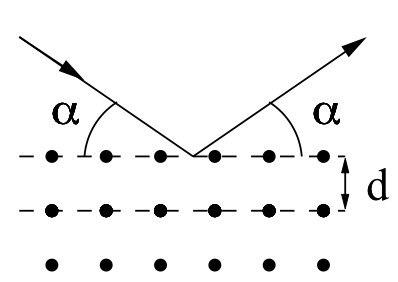
\includegraphics[width=0.3\textwidth]{plots/bragg.jpg}
    \caption{Darstellung der Bragg-Reflexion an einem Gitter mit der
    Gitterkonstante $d$ und dem Bragg-Winkel $\alpha$.\cite[3]{anleitung}}
\end{figure}
\\Die Röntgenstrahlung ist auf zwei Effekt zurückzuführen.
\subsubsection*{Kontinuierliches Spektrum}
Beim Auftreffen der Elektronen auf das Anodenmaterial wird dieses ionsisiert, sodass
ein gebundenes Elektron von einer höheren Schale auf eine niedrigere Schale fallen kann und dabei
Energie in Form von Röntgenquanten imitiert. Die abgestrahlte Energie entspricht dann der Differenz
der Energieniveaus.
\begin{equation}
    h\cdot v=E_m-E_n
\end{equation}
Das charakteristische Spektrum ist vom Anodenmaterial abhängig und zeichnet sich im
Röntgenspektrum durch schwarfe Linien aus.
Für ein Elektron in einem Mehrelektronenatom ergibt sich die Energie durch
\begin{equation}
    E_n=-R_{\infty}\cdot z_{eff}^2 \cdot \frac{1}{n^2},
\end{equation}
wobei die Rydbergenergie $R_{\infty}=13.6$eV und die effektive Kernladung 
$z_{eff}=z-\sigma$ mit der Abschirmkonstante $\sigma$ ist.
\begin{figure}
    \centering
    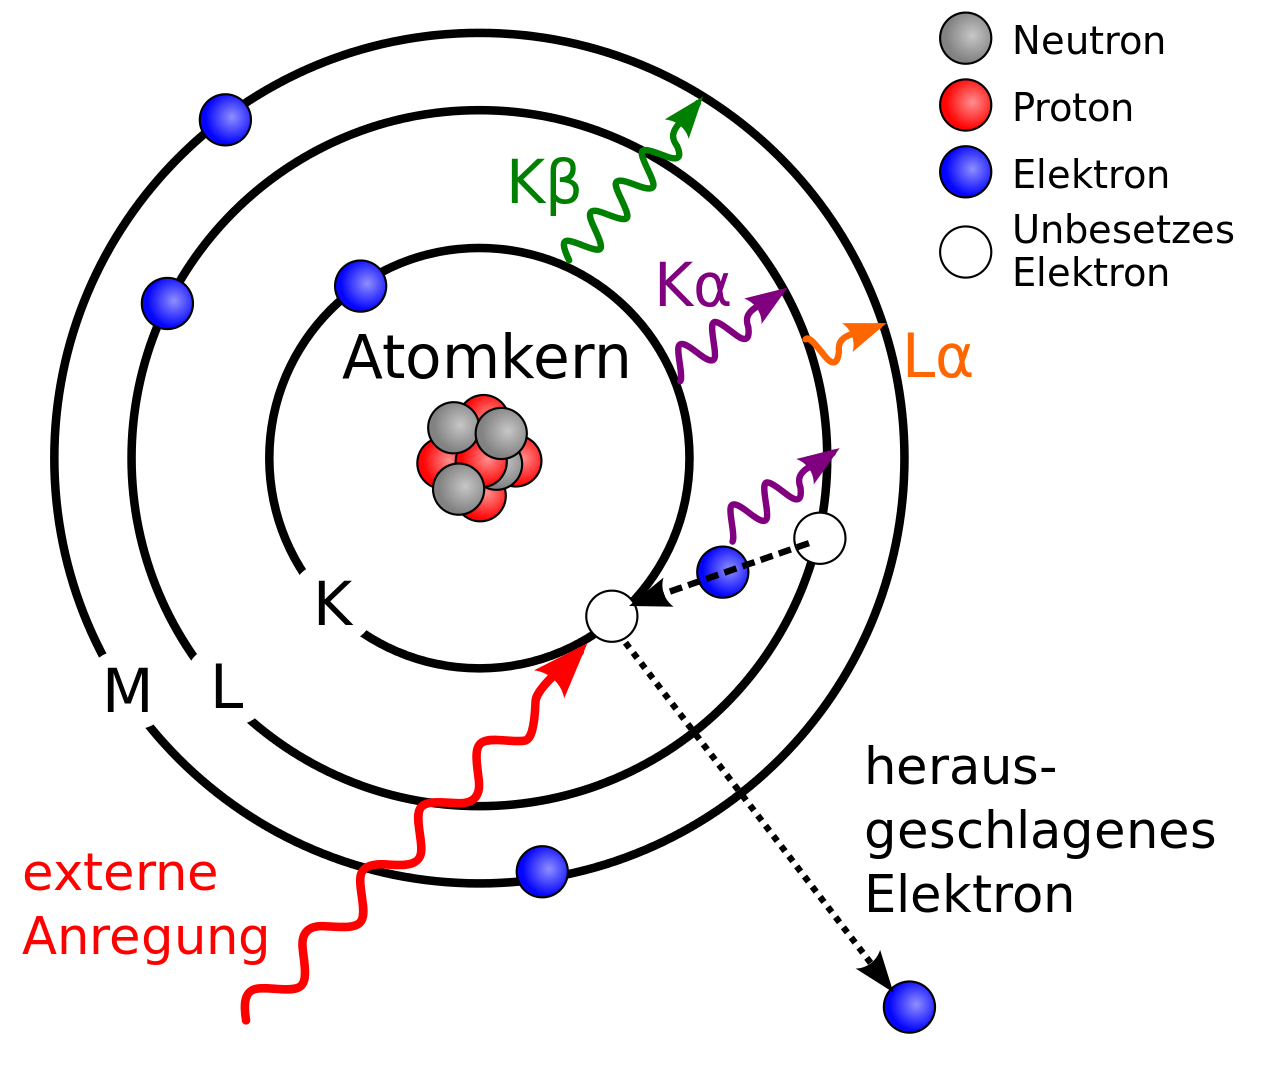
\includegraphics[width=0.4\textwidth]{plots/chS.png}
    \caption{Darstellung des Prozesses der Röntenemission durch die
    Ionisation des Atoms. Das (Röntgen)Photon wirkt als exteren Anregung, welches
    ein Elektron aus der inneren Schale schlägt. Ein anderes Elektron aus einer
    höheren Schale rutscht nach und gibt Energie in Form von Strahlung ab.\cite{wiki}}
\end{figure}
\subsubsection*{Bremsstrahlung}
Durch Abbremsen der freien Elektronen in einem Elektrischen Feld 
wird Energie durch Röntgenquanten frei. Die Energie entspricht dabei
dem Energieverlust der Abbremsung. Bei vollständiger Abbremsung ergibt
sich die Wellenlänge
\begin{equation}
    \lambda_{min}=\frac{h \cdot c}{e_0U}.
    \label{eqn:minW}
\end{equation}
Da hierbei verschieden hohe kinetische Energien abgegeben werden können,
äußert siche die Bremsstrahlung im Spektrum durch einen Kontinuierlichen
Verlauf.
\subsection{Halbwertsbreite (Full Width at Half Maximum)}
Die Breite bie halber Höhe (kurz: FWHM) beschreibt "die Differenz zwischen 
den beiden Argumentwerten, für die die Funktionswerte auf die 
Hälfte des Maximums abgesunken sind."\cite{wiki2}
\begin{figure}
    \centering
    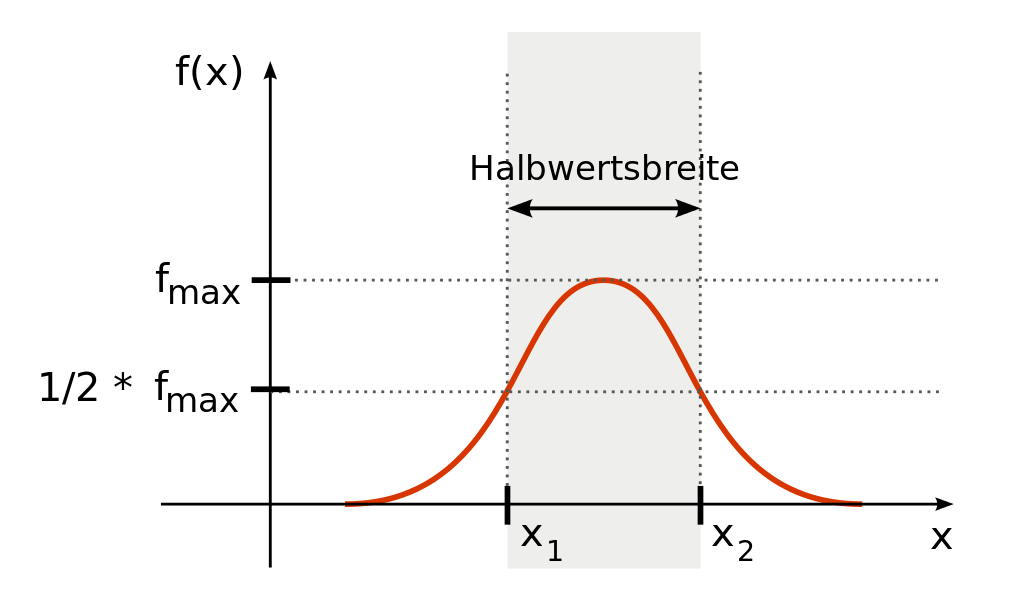
\includegraphics[width=0.4\textwidth]{plots/Halbwertsbreite.png}
    \caption{}
\end{figure}
\subsection{Absorbtion}
Treffen Röntgenstrahlen auf ein Material, so nimmt dieses die Strahlung zum Teil
auf (Absorbtion). Diese ist zum Teil vom Material, derer Dicke $d$ und der Energie 
der Strahlung abhängig.
\begin{equation}
    \frac{I(d)}{I_0}=e^{-\mu d}=:\tau
\end{equation}
Dabei ist $\mu$ der Absorbtionskoeffizient.\\
Dieser ist abhängig von der Energie der Strahlung und nimmt bei zunehmender
Strahlungsenergie ab. $\mu$ steigt sprunghaft an, wenn die Strahlungsenergie
gleich groß der Bindungsenergie eines Elektrons aus der nächsten inneren Schale ist.
Man spricht von einer Absorbtinskante.
Für die K-Kante (n=1) ergibt sich nach der Sommerfledschen Feinstrukturformel
die Abschirmkonstante
\begin{equation}
    \sigma_K=Z-\sqrt{\frac{E_K}{R_{\infty}}-\frac{\alpha^2Z^4}{4}}
\end{equation}
Bei Strahlungsenergien unterhalb von $1$MeV treten erstmal Compton- und Photoeffekt ein.



